\documentclass[10pt,a4paper]{article}
\usepackage[utf8]{inputenc}
\usepackage[T1]{fontenc}
\IfFileExists{brazil.ldf}{\usepackage[brazil]{babel}}{}
\usepackage{charter}
\usepackage[a4paper,top=1.35cm,bottom=1.45cm,left=1.55cm,right=1.55cm,footskip=0.7cm]{geometry}
\usepackage{microtype}
\usepackage{amsmath}
\usepackage{booktabs}
\usepackage{tabularx}
\usepackage{enumitem}
\usepackage[dvipsnames]{xcolor}
\usepackage{titlesec}
\usepackage{fancyhdr}
\usepackage[hidelinks]{hyperref}
\usepackage{tikz}
\usetikzlibrary{positioning, arrows.meta}
\usepackage{pgfplots}
\pgfplotsset{compat=1.18}
\usepackage{xstring}

% =====================================================================
% numeros_finais.tex
% Gerado pelo pipeline (scripts/gerar_numeros_latex.py) apos o corte.
% NAO editar a mao: rodar o script e recompilar o PDF.
% =====================================================================
\newcommand{\statusprevisao}{FINAL (corte 03/10/2026 20h00)}
\newcommand{\npesquisas}{6}
\newcommand{\listapesquisas}{Datafolha (BR-00304/2026 e BR-08039/2026), Quaest (BR-06520/2026), PoderData (BR-01739/2026), AtlasIntel (BR-04391/2026) e Real Time Big Data (BR-09503/2026)}

% Modelo oficial (votos validos, %)
\newcommand{\pLula}{45,6}
\newcommand{\pFlavio}{45,9}
\newcommand{\pCury}{2,6}
\newcommand{\pCaiado}{2,6}
\newcommand{\pRenan}{2,5}
\newcommand{\pZema}{0,7}
\newcommand{\pSamara}{0,1}
\newcommand{\pClariana}{0,0}
\newcommand{\pEdmilson}{0,0}
\newcommand{\pHertz}{0,0}
\newcommand{\pRui}{0,0}
\newcommand{\pWilson}{0,0}

% M0 puro (sensibilidade)
\newcommand{\mLula}{45,4}
\newcommand{\mFlavio}{41,5}
\newcommand{\mCury}{4,1}
\newcommand{\mCaiado}{3,0}
\newcommand{\mRenan}{3,9}
\newcommand{\mZema}{1,1}

% Aba 2
\newcommand{\pAbst}{22,3}
\newcommand{\pBrancos}{1,6}
\newcommand{\pNulos}{2,8}


\definecolor{azul}{HTML}{1F3A5F}
\definecolor{cinza}{HTML}{555555}

\titleformat{\section}{\normalfont\bfseries\color{azul}}{\thesection.}{0.5em}{}
\titlespacing*{\section}{0pt}{4pt}{1pt}
\setlist{nosep,leftmargin=1.2em,topsep=1pt}
\setlength{\parindent}{0pt}
\setlength{\parskip}{2.5pt}
\renewcommand{\arraystretch}{1.03}
\setlength{\tabcolsep}{3.5pt}

\pagestyle{fancy}
\fancyhf{}
\renewcommand{\headrulewidth}{0pt}
\fancyfoot[L]{\footnotesize\color{cinza}Desafio de Estatística e Econometria, FGV EPGE}
\fancyfoot[R]{\footnotesize\color{cinza}\thepage/2}

\newcommand{\pp}{\,p.p.}

% Bloco StrSubstitute para pgfplots
\StrSubstitute{\pFlavio}{,}{.}[\pFlavioDot]
\StrSubstitute{\pLula}{,}{.}[\pLulaDot]
\StrSubstitute{\pCury}{,}{.}[\pCuryDot]
\StrSubstitute{\pCaiado}{,}{.}[\pCaiadoDot]
\StrSubstitute{\pRenan}{,}{.}[\pRenanDot]
\StrSubstitute{\pZema}{,}{.}[\pZemaDot]
\StrSubstitute{\mFlavio}{,}{.}[\mFlavioDot]
\StrSubstitute{\mLula}{,}{.}[\mLulaDot]
\StrSubstitute{\mCury}{,}{.}[\mCuryDot]
\StrSubstitute{\mCaiado}{,}{.}[\mCaiadoDot]
\StrSubstitute{\mRenan}{,}{.}[\mRenanDot]
\StrSubstitute{\mZema}{,}{.}[\mZemaDot]

\begin{document}

{\large\bfseries\color{azul} Previsão do 1º turno presidencial de 2026: nota metodológica}\\[2pt]
{\small João Pedro Valuche de Andrade Pereira \textbullet\ Lethicia Manfioletti Possamai \textbullet\ Arthur Caron Lyra}\\[3pt]
\colorbox{azul!8}{\parbox{\dimexpr\linewidth-2\fboxsep}{\small
\textbf{Horário de corte dos dados: sábado, 03/10/2026, às 20h00 (horário de Brasília).} Nenhuma pesquisa divulgada após esse horário entrou na previsão. Status destes números: \statusprevisao.}}

\vspace{1pt}

\section{Objetivo}
Projetamos a distribuição de votos válidos para os doze candidatos a presidente da República e os percentuais de abstenção, votos brancos e votos nulos no primeiro turno da eleição presidencial de 2026. Avaliamos o desempenho dos modelos por meio do erro absoluto médio (MAE) calculado sobre todos os candidatos da cédula eleitoral. Optamos por incluir todas as candidaturas porque distorções em concorrentes menores alteram a soma total dos votos e desvios pontuais em qualquer candidato geram o mesmo impacto na precisão da estimativa.

\section{Dados e pipeline}
\begin{figure}[htbp]
\centering
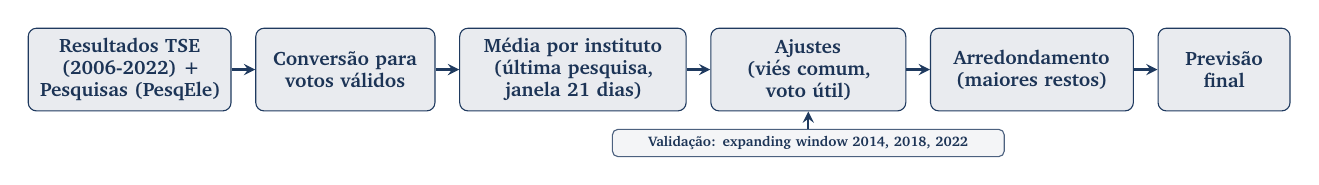
\begin{tikzpicture}[
    node distance=0.30cm,
    caixa/.style={
        rectangle, rounded corners=3pt,
        draw=azul, fill=azul!10, text=azul!90!black,
        align=center, font=\scriptsize\bfseries,
        inner sep=2.5pt, minimum height=1.05cm
    },
    seta/.style={->, >=stealth, thick, color=azul},
    faixa/.style={
        rectangle, rounded corners=2pt,
        draw=azul!80, fill=azul!5, text=azul!90!black,
        align=center, font=\tiny\bfseries,
        inner sep=2.5pt
    }
]
\node[caixa, text width=2.4cm] (tse) {Resultados TSE\\(2006-2022) +\\Pesquisas (PesqEle)};
\node[caixa, text width=2.1cm, right=of tse] (conv) {Conversão para\\votos válidos};
\node[caixa, text width=2.7cm, right=of conv] (media) {Média por instituto\\(última pesquisa,\\janela 21 dias)};
\node[caixa, text width=2.3cm, right=of media] (ajust) {Ajustes\\(viés comum,\\voto útil)};
\node[caixa, text width=2.4cm, right=of ajust] (arred) {Arredondamento\\(maiores restos)};
\node[caixa, text width=1.5cm, right=of arred] (prev) {Previsão\\final};

\draw[seta] (tse) -- (conv);
\draw[seta] (conv) -- (media);
\draw[seta] (media) -- (ajust);
\draw[seta] (ajust) -- (arred);
\draw[seta] (arred) -- (prev);

\node[faixa, below=0.22cm of ajust, text width=4.8cm] (val) {Validação: expanding window 2014, 2018, 2022};
\draw[seta] (val) -- (ajust);
\end{tikzpicture}
\vspace{-4pt}
\caption{Diagrama do pipeline metodológico e protocolo de validação temporal. Fonte: elaboração própria.}
\label{fig:pipeline}
\end{figure}

Coletamos os resultados oficiais apurados pelo Tribunal Superior Eleitoral (TSE) de 2006 a 2022 e 109 pesquisas estimuladas de primeiro turno divulgadas nos 21 dias que antecederam cada eleição. Para a eleição de 2026, compilamos as \npesquisas{} pesquisas registradas no TSE divulgadas até o horário de corte: \listapesquisas. Estabelecemos a janela de 21 dias porque as decisões de voto dos eleitores se estabilizam nas semanas finais de campanha. Mantivemos unicamente a última pesquisa de cada instituto com o intuito de evitar que empresas com rodadas diárias de rastreamento exerçam peso desmedido no resultado agregado.

\section{Modelos e protocolo de validação}
Calculamos a proporção inicial de votos válidos de cada levantamento excluindo abstenções, brancos, nulos e indecisos:
\begin{equation}
v_{i,j} = \frac{x_{i,j}}{\sum_{c=1}^{K} x_{c,j}}
\end{equation}
em que $x_{i,j}$ representa a intenção divulgada para o candidato $i$ pelo instituto $j$.

Formulamos quatro especificações base de agregação. O modelo M0 computa a média simples entre os $J$ institutos da eleição:
\begin{equation}
p_{i}^{\text{M0}} = \frac{1}{J}\sum_{j=1}^{J} v_{i,j}
\end{equation}
O modelo M1 atribui pesos ponderados pela raiz quadrada do tamanho amostral $N_j$ e pelo decaimento temporal exponencial com meia-vida $h$:
\begin{equation}
w_j = \sqrt{N_j} \cdot 2^{-\Delta t_j / h}, \quad p_i^{\text{M1}} = \frac{\sum_{j} w_j v_{i,j}}{\sum_j w_j}
\end{equation}
O modelo M2 corrige o viés sistemático de cada instituto (\emph{house effect}) por bloco político, aplicando encolhimento bayesiano:
\begin{equation}
\hat\beta_{j,b} = \frac{n_j}{n_j + k}\bar\beta_{j,b}, \quad v_{i,j}^{\text{corr}} = v_{i,j} - \hat\beta_{j,b(i)}
\end{equation}
O modelo M3 estima uma regressão Ridge com regularização $L_2$ sobre a média das pesquisas, incumbência e ordenamento prévio:
\begin{equation}
\hat\beta^{\text{Ridge}} = \arg\min_\beta \left\{ \sum_{t} (y_t - X_t\beta)^2 + \alpha \|\beta\|_2^2 \right\}
\end{equation}

Mensuramos o erro preditivo por meio do MAE sobre os $K$ candidatos da apuração:
\begin{equation}
\text{MAE} = \frac{1}{K}\sum_{i=1}^{K} |p_i - r_i|
\end{equation}
onde $r_i$ é o percentual oficial apurado pelo TSE.

Adotamos a validação temporal prospectiva (\emph{expanding window}) nos pleitos de 2014, 2018 e 2022 porque esse critério impede o uso de informações do futuro para calibrar previsões passadas. Fixamos a regra de decisão antes da execução do backtest para coibir escolhas discricionárias após a verificação dos erros. Uma especificação de maior complexidade só é admitida se a diminuição média do MAE for superior ao erro-padrão amostral das diferenças:
\begin{equation}
\bar\Delta > \text{EP}(\Delta) = \frac{s_\Delta}{\sqrt{n}}
\end{equation}
Em caso de empate estatístico, preservamos a formulação de menor complexidade.

\begin{center}\small
\textbf{Tabela 1:} Avaliação dos modelos e ajustes no backtest expanding window (MAE em p.p.).\\[2pt]
\begin{tabular}{lccccl}
\toprule
\textbf{Etapa 1: modelo base} (melhor configuração) & \textbf{2014} & \textbf{2018} & \textbf{2022} & \textbf{Média} & \textbf{Decisão} \\
\midrule
M0 média simples & 1,33 & 1,50 & 0,83 & \textbf{1,22} & escolhido \\
M1 recência ($h=7$) & 1,96 & 1,73 & 0,77 & 1,49 & rejeitado \\
M2 \emph{house effect} ($k=10$) & 2,09 & 1,84 & 0,82 & 1,58 & rejeitado \\
M3 Ridge ($\alpha=1$) & 1,85 & 2,02 & 1,19 & 1,69 & rejeitado \\
\midrule
\textbf{Etapa 2: ajustes sobre o M0} & & & & & \textbf{$\bar\Delta$ / EP} \\
\midrule
+ viés comum ($k_\mu=3$) & 0,95 & 1,45 & 0,71 & 1,04 & 0,18 / 0,10 \\
+ voto útil ($\gamma=1$) & 1,31 & 1,43 & 0,53 & 1,09 & 0,13 / 0,09 \\
+ histórico dos nanicos ($w=0{,}5$) & 1,31 & 1,50 & 0,84 & 1,22 & 0,00 / 0,01 \\
\textbf{Modelo final} (M0 + viés comum + voto útil) & 0,92 & 1,39 & 0,58 & \textbf{0,96} & 0,26 / 0,04 \\
\bottomrule
\end{tabular}\\[2pt]
{\footnotesize MAE sobre todos os candidatos da urna (11 a 13). No LOEO, o modelo final tem MAE de 1,24 contra 1,45 do M0, e melhora em 4 de 5 eleições. Fonte: elaboração própria.}
\end{center}

\section{Modelo final}
Incorporamos dois ajustes econométricos sobre a média simples M0 selecionada no backtest. O primeiro corrige o viés comum médio das pesquisas em cada bloco político $b$, aplicando encolhimento bayesiano sobre o erro histórico médio das pesquisas em relação à urna:
\begin{equation}
\hat\mu_b = \frac{N}{N+3}\cdot\frac{1}{N}\sum_{t=1}^{N} \left(\bar v^{\,\text{pesq}}_{b,t} - v^{\text{TSE}}_{b,t}\right)
\end{equation}
onde $N$ indica a quantidade de eleições no conjunto de treino. Introduzimos esse ajuste porque os institutos compartilham metodologias amostrais semelhantes que subestimaram recorrentemente o principal opositor do partido governista nas vésperas das eleições recentes.

O segundo ajuste captura a coordenação estratégica de voto útil na reta final. Calculamos a perda média $\bar\delta$ verificada conjuntamente pelo terceiro e quarto colocados nas eleições passadas e a transferimos proporcionalmente aos dois concorrentes líderes:
\begin{equation}
\Delta v_i = \bar\delta \cdot \frac{p_i}{p_1 + p_2}, \quad i \in \{1, 2\}
\end{equation}
Fundamentamos esse mecanismo na decisão de eleitores que abandonam concorrentes sem probabilidade de segundo turno para definir a disputa imediata entre os favoritos.

Finalizadas as correções, renormalizamos as frações para cumprir a restrição orçamentária probabilística e executamos o algoritmo dos maiores restos (método de Hamilton) para assegurar o fechamento exato em 100,0\% com uma casa decimal:
\begin{equation}
\sum_{i=1}^{12} \hat p_i = 100{,}0\%
\end{equation}
Testamos também uma âncora histórica calibrada na mediana de votação de legendas equivalentes no TSE, mas descartamos a medida porque a redução de erro foi nula no backtest ($w=0$).

\section{Resultados de 2026}
\begin{center}\small
\textbf{Tabela 2:} Previsão de votos válidos para 2026 (modelo final e média simples M0).\\[2pt]
\begin{tabular}{lcc@{\hspace{2.2em}}lcc}
\toprule
\textbf{Candidato} & \textbf{Final} & \textbf{M0} & \textbf{Candidato} & \textbf{Final} & \textbf{M0} \\
\midrule
Flávio Bolsonaro (PL) & \textbf{\pFlavio} & \mFlavio & Romeu Zema (Novo) & \pZema & \mZema \\
Luiz Inácio Lula da Silva (PT) & \textbf{\pLula} & \mLula & Samara Martins (UP) & \pSamara & \\
Augusto Cury (Avante) & \pCury & \mCury & Clariana Barão (DC) & \pClariana & \\
Ronaldo Caiado (PSD) & \pCaiado & \mCaiado & Edmilson Costa (PCB) & \pEdmilson & \\
Renan Santos (Missão) & \pRenan & \mRenan & Hertz Dias (PSTU) & \pHertz & \\
 & & & Rui Costa Pimenta (PCO) & \pRui & \\
 & & & Wilson Grassi (Democrata) & \pWilson & \\
\bottomrule
\end{tabular}\\[2pt]
{\footnotesize Projeções em \% de votos válidos. A coluna M0 é a média simples das pesquisas, mostrada para transparência. Fonte: elaboração própria.}
\end{center}

\begin{figure}[htbp]
\centering
\begin{tikzpicture}
\begin{axis}[
    ybar,
    bar width=6.5pt,
    width=0.96\linewidth,
    height=3.8cm,
    ymin=0, ymax=52,
    ylabel={Votos válidos (\%)},
    symbolic x coords={Flavio, Lula, Cury, Caiado, Renan, Zema},
    xtick=data,
    xticklabels={Flávio, Lula, Cury, Caiado, Renan, Zema},
    legend style={at={(0.98,0.95)}, anchor=north east, font=\scriptsize},
    nodes near coords,
    nodes near coords style={font=\tiny},
    ymajorgrids=true,
    grid style={dashed, gray!30},
    axis line style={cinza!50},
    tick label style={font=\scriptsize},
    label style={font=\scriptsize},
    enlarge x limits=0.12,
]
\addplot[fill=azul!85, draw=azul] coordinates {
    (Flavio, \pFlavioDot)
    (Lula, \pLulaDot)
    (Cury, \pCuryDot)
    (Caiado, \pCaiadoDot)
    (Renan, \pRenanDot)
    (Zema, \pZemaDot)
};
\addplot[fill=cinza!40, draw=cinza] coordinates {
    (Flavio, \mFlavioDot)
    (Lula, \mLulaDot)
    (Cury, \mCuryDot)
    (Caiado, \mCaiadoDot)
    (Renan, \mRenanDot)
    (Zema, \mZemaDot)
};
\legend{Modelo final, Média simples M0}
\end{axis}
\end{tikzpicture}
\vspace{-6pt}
\caption{Projeções de votos válidos (\%) para os principais candidatos em 2026: modelo final versus média simples M0. Fonte: elaboração própria.}
\label{fig:projecoes}
\end{figure}

A diferença projetada entre os dois primeiros candidatos (\pFlavio\% para Flávio Bolsonaro contra \pLula\% para Luiz Inácio Lula da Silva) é de 0,3 p.p., magnitude inferior ao erro médio observado para a margem entre os dois concorrentes mais votados no backtest histórico (média de 4,5 p.p. no modelo final, com $n=3$). Concluímos que as estimativas configuram um quadro de disputa indefinida entre as duas lideranças, sem base amostral para antecipar o vencedor do primeiro turno.

Registramos uma limitação relevante relativa à aplicação do viés comum. Na validação de 2022, esse ajuste reduziu o MAE global de 0,83 para 0,58 p.p., porém superestimou a votação do concorrente opositor (44,8\% frente a 43,2\% na urna) e agravou o erro da margem entre os líderes de 1,3 para 4,3 p.p. Conservamos o viés comum porque a nossa regra pré-estabelecida visa minimizar o erro médio da distribuição integral dos candidatos, mas ressaltamos que a correção pode gerar desvio na margem em eleições cujo comportamento divirja do histórico das três rodadas anteriores.

\section{Abstenção, brancos e nulos}
Comparamos três métodos por validação temporal expanding window: persistência do resultado anterior, média móvel histórica e tendência linear, adotando a ordem de parcimônia persistência, média e tendência. Calculamos a taxa de abstenção em relação ao colégio de eleitores aptos, e os votos brancos e nulos em relação ao comparecimento efetivo às urnas.

\begin{center}\small
\textbf{Tabela 3:} Backtest e seleção de método para agregados eleitorais (2014-2022).\\[2pt]
\begin{tabular}{lccccl}
\toprule
\textbf{Variável} & \textbf{Persistência} & \textbf{Média} & \textbf{Tendência} & \textbf{Previsão} & \textbf{Decisão} \\
\midrule
Abstenção & 0,94 & 2,17 & \textbf{0,40} & \textbf{\pAbst\%} & tendência vence ($\bar\Delta=-0{,}54$; EP $=0{,}36$) \\
Brancos & \textbf{0,99} & 1,00 & 1,21 & \textbf{\pBrancos\%} & empate, vence persistência \\
Nulos & \textbf{1,32} & 1,21 & 1,40 & \textbf{\pNulos\%} & empate ($\bar\Delta=-0{,}10$; EP $=0{,}14$), persistência \\
\bottomrule
\end{tabular}\\[2pt]
{\footnotesize MAE médio em pontos percentuais nas eleições de 2014, 2018 e 2022. Fonte: elaboração própria.}
\end{center}

Observamos que o movimento persistente de crescimento da abstenção (de 16,8\% em 2006 para 21,0\% em 2022) justifica a superioridade empírica da tendência linear, ao passo que a forte redução recente de brancos e nulos sob polarização acentuada faz com que a persistência imediata reflita a conjuntura presente melhor do que médias de períodos mais extensos.

\section{Reprodutibilidade}
Disponibilizamos os códigos, bases processadas, documentação metodológica e rotinas de validação em \url{https://github.com/pvaluche/trabalho-econometria-a1/tree/entrega-final}. Todas as projeções e tabelas constantes nesta nota são compiladas diretamente pelos procedimentos computacionais do projeto a partir dos dados originais.

\end{document}
